% 2026-03-31_pflichtteile.tex
% lualatex 2026-03-31_pflichtteile.tex
% dvisvgm --no-fonts 2026-03-31_pflichtteile.dvi

\documentclass[tikz,border=10pt]{standalone}
\usepackage[T1]{fontenc}
\usepackage{lmodern}
\renewcommand{\familydefault}{\sfdefault}
\usepackage{amsmath}

\usetikzlibrary{positioning, calc, decorations.pathreplacing}

\definecolor{nodebk}{HTML}{111111}
\definecolor{annred}{HTML}{c0392b}
\definecolor{edgegray}{HTML}{444444}

%% Makro: \quotannot{Anker}{Zähler1}{Nenner1}{Zähler2}{Nenner2}{Zähler3}{Nenner3}
%% linker Bruch schwarz, rechter Bruch + Ergebnis rot
\newcommand{\quotannot}[7]{%
  \node[draw=none, below=0.10cm of #1] (#1p)
    {{\color{nodebk}$\dfrac{#2}{#3}$} $\cdot$ {\color{annred}$\dfrac{#4}{#5}$}};
  \draw[decorate,
        decoration={brace, amplitude=4pt, mirror},
        color=annred, line width=1.0pt]
    (#1p.south west) -- (#1p.south east);
  \node[draw=none, color=annred, below=0.20cm of #1p]
    {$\dfrac{#6}{#7}$};
}

\begin{document}
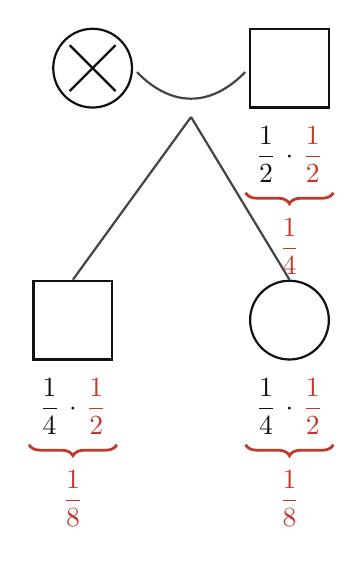
\begin{tikzpicture}[
  thick,
  every node/.style={draw=black, thick, color=nodebk},
  font=\sffamily
]

  %% ── Elterngeneration ──────────────────────────────────────────
  % Verstorbener: Kreis mit X
  \node[circle, minimum size=1.0cm] (erb) at (0,0) {};
  \draw[color=nodebk, thick]
    ($(erb.north west)!0.1!(erb.south east)$) -- ($(erb.north west)!0.9!(erb.south east)$)
    ($(erb.north east)!0.1!(erb.south west)$) -- ($(erb.north east)!0.9!(erb.south west)$);

  % Ehegatte: Rechteck
  \node[rectangle, minimum size=1.0cm] (ehe) at (2.5,0) {};

  %% ── Kindergeneration ──────────────────────────────────────────
  % Sohn: Rechteck
  \node[rectangle, minimum size=1.0cm] (sohn) at (-0.25, -3.2) {};
  % Tochter: Kreis
  \node[circle,    minimum size=1.0cm] (toch) at ( 2.5,  -3.2) {};

  %% ── Verbindungslinien ─────────────────────────────────────────
  % Geschwungene Linie zwischen Eltern
  \draw[color=edgegray, shorten >=2pt, shorten <=2pt]
    (erb.east) .. controls (1.0, -0.5) and (1.5, -0.5) .. (ehe.west);

  % Mittelpunkt als Ursprung der Kindslinien
  \coordinate (mid) at (1.25, -0.62);

  \draw[color=edgegray] (mid) -- (sohn.north);
  \draw[color=edgegray] (mid) -- (toch.north);

  %% ── Annotationen ──────────────────────────────────────────────
  %                    Anker  Z1  N1  Z2  N2  Z3  N3
  \quotannot{ehe} {1}{2}{1}{2}{1}{4}
  \quotannot{sohn}{1}{4}{1}{2}{1}{8}
  \quotannot{toch}{1}{4}{1}{2}{1}{8}

\end{tikzpicture}
\end{document}